\graphicspath{{figures/chapter1/}}
\onehalfspacing

\chapter{Introduction}\label{ch:1}

\vfill

\newthought{This chapter is based on:}

\noindent 

\begin{itemize}
    \item De Gaetani, C. I., Ioli, F., \& Pinto, L. (2021). Aerial and UAV Images for Photogrammetric Analysis of Belvedere Glacier Evolution in the Period 1977–2019. Remote Sensing, 13(18), 3787. \url{https://doi.org/10.3390/rs13183787}
    \item Ioli, F., Bianchi, A., Cina, A., De Michele, C., Maschio, P., Passoni, D., \& Pinto, L. (2021). Mid-Term Monitoring of Glacier’s Variations with UAVs: The Example of the Belvedere Glacier. Remote Sensing, 14(1), 28. \url{https://doi.org/10.3390/rs14010028}
    \item Ioli, F., Dematteis, N., Giordan, D., Nex, F., Pinto, L. (2024). Deep Learning Low-cost Photogrammetry for 4D Short-term Glacier Dynamics Monitoring. \textit{PFG}. \url{https://doi.org/10.1007/s41064-023-00272-w}
\end{itemize}

\newpage

\section{Motivation and relevance}

Glaciers worldwide are experiencing profound transformations due to the ongoing climate crisis~\citep{Oerlemans2005}, and their sensitivity to temperature fluctuations renders them powerful indicators of global climate change~\citep{Barry2006}.
Alpine glaciers in temperate zones are particularly susceptible to rising temperatures. The accelerated rate of glacial retreat underscores the necessity for comprehensive monitoring programs~\citep{Zemp2006, Sommer2020}. 
Therefore, they are often considered as a proxy for climate change evaluation.
Projections point out that the European Alps may lose more than 60\% of ice volume by the end of the century under the RCP2.6 scenario, whereas a more significant amount of ice loss is expected under worse scenarios~\citep{Zekollari2019}.

However, mountain glaciers are a critical component of the local economy regarding hydroelectric production, tourist activities, and freshwater supply~\citep{Barnett2005, hock2005}. 
Additionally, glacier melting and retreat are triggering several glaciological processes, e.g., ice break-off, glacier outburst, snow/ice avalanches, and gravitational slope stability processes, such as rockfalls and collapses, and debris flow, which can threaten the population infrastructure of the nearby urban areas~\citep{Kaab2004, Deline2015, Giordan2020}.

In the European Alps, the number of mass movements and hazardous events in high-elevation environments has experienced an increase in the past decade due to climate change \citep{chiarle2023, Nigrelli2024}.
A relevant and tragic example was the collapse of a section of the Marmolada Glacier (Dolomites, Italy), which occurred on July 3, 2022, at 13:43:20 CEST\footnote{\url{https://www.theguardian.com/world/2022/jul/03/deaths-glacier-breaks-marmolada-mountain-italy}}. 
The collapse caused an ice avalanche that killed 11 mountaineers trying to reach the Marmolada summit and injured 7~\citep{Olivieri2023, Bondesan2023}.
The collapse occurred on the northern slope of the glacier at an elevation of \SI{3213}{\masl} and involved a volume of \SI{\sim 96000}{\cubic\meter}~\citep{Olivieri2023}.
The detachment was caused by a failure along a median crevasse, partially filled by meltwater due to highly anomalous temperatures, that reached \SI{10.7}{\celsius} at the time of the event.
The sudden glacier collapse was probably induced by hydraulic jacking and pressure within a thin layer of basal till~\citep{Bondesan2023}.

Just one year after the Marmolada collapse, another relevant slope instability event was registered in the Austrian state of Tyrol, close to the Italian border. 
On June 11, 2023, a significant portion of the summit of Fluchthorn, a nearly \SI{3400}{\masl} collapsed, causing more than \SI{100000}{\cubic\meter} of rock to crash into the valley and triggering mudslides\footnote{\mbox{\url{https://edition.cnn.com/2023/06/14/europe/austrian-mountain-fluchthorn-rockslide-climate-intl/index.html}}}.
This event was likely related to the thawing permafrost due to the high temperatures of that period\footnote{\url{https://blogs.agu.org/landslideblog/2023/06/12/fluchthorn-1/}}.

\begin{figure}[ht!]
    \centering
    \subcaptionbox{}{
        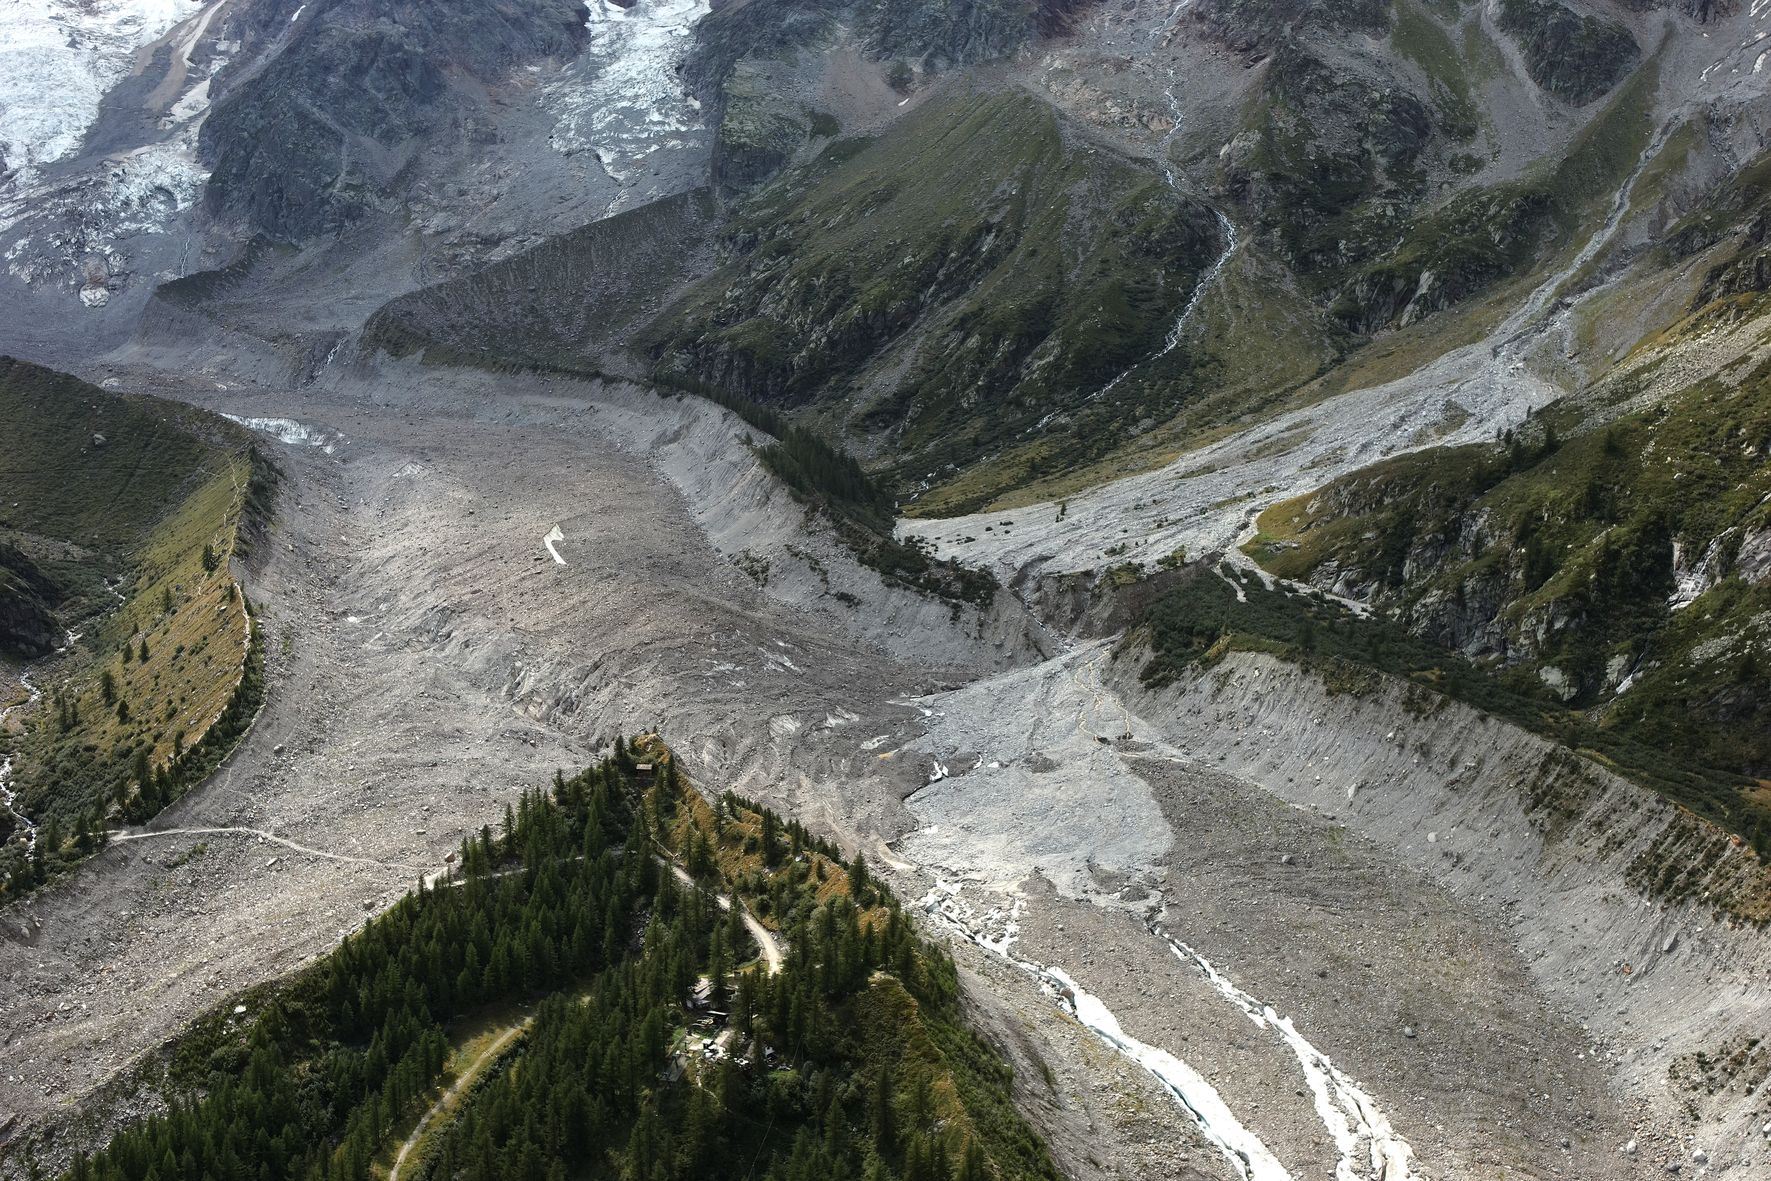
\includegraphics[height=4.8cm]{DJI_20230830144913_0181}
    }
    \subcaptionbox{\label{fig:1:belvedere_debris_flow:cam}}{
        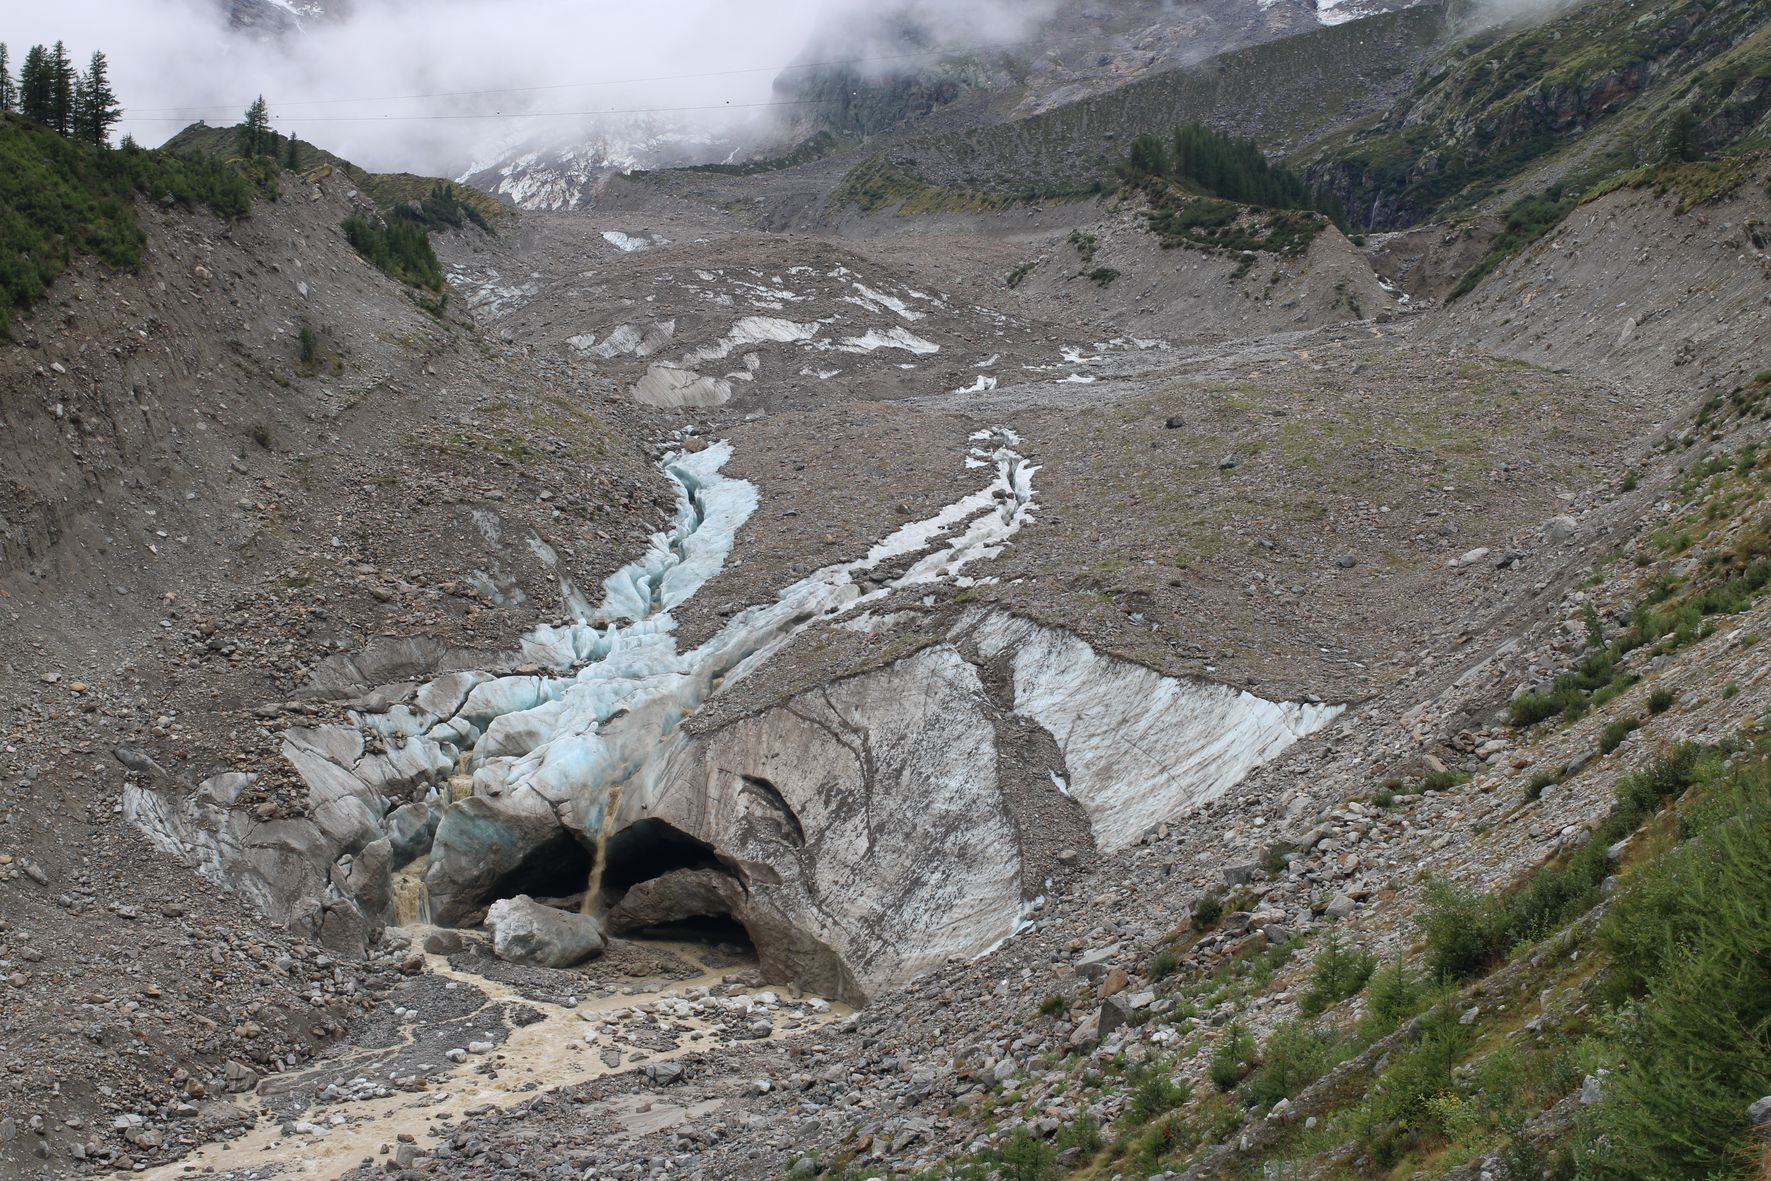
\includegraphics[height=4.8cm]{p1_20230828_155946_IMG_1457.jpg}
    }
    \caption{Impact of the August 27, 2023 debris flow on the Belvedere Glacier (Anscasca Valley, Italian Alps). \textbf{(a)} Aerial view acquired (August 30, 2023, author's photo) reveals the extent of debris accumulation within the Castelfranco gully and across the glacier's northern lobe; \textbf{(b)} Picture of the Belvedere Glacier northern lobe few hours after the debris flow event (August 28, 2023, 4:00 PM), captured by the fixed monitoring system. Note the 
    muddy channels carved into the glacier's surface. These channels are remnants of the powerful flow that washed away much of the debris.
    }
    \label{fig:1:belvedere_debris_flow}
\end{figure}

On August 27, 2023, a large debris flow occurred at the Belvedere Glacier (Anzasca Valley, Italian Alps)\footnote{\url{https://www.regione.piemonte.it/web/temi/protezione-civile-difesa-suolo-opere-pubbliche/protezione-civile/sorvolo-ghiacciai-monte-rosa-07092023}}.
The debris flow was triggered at the beginning of the steep Castelfranco gully, located at approximately \SI{3600}{\masl} on the streamwise-left side of the Belvedere Glacier northwest lobe (\figref{fig:1:belvedere_debris_flow}).
During the event, a volume of \SI{\sim 200000}{\cubic\meter} was accumulated on top of the Belvedere Glacier and obstructed the sinkhole that allowed the Castelfranco stream to flow below the ice sheet. 
This caused the water to stream on top of the glacier, carving deep grooves on the Belvedere Glacier (\figref{fig:1:belvedere_debris_flow:cam}). 
A large portion of the debris cumulated in the riverbed was transported towards the municipality of Macugnaga by the river Anza.
A previous event with similar characteristics but significantly smaller dimensions occurred in 2008 and was documented by \citet{Mortara2009}, who reported an estimation of a few thousand cubic meters of cumulated debris volume.

In this context, a systematic monitoring of glaciers and related glaciological processes assumes a crucial significance.
To thoroughly understand these complex systems, accurate observations are essential \citep{Kaab2005}.
A particular focus is usually placed on monitoring surface kinematics, as these can potentially offer early warning signs of impending instability or collapse events \citep{Faillettaz2015}.
Nevertheless, monitoring glaciers in remote areas and inaccessible terrains often presents logistical and safety challenges.
Therefore, remote sensing techniques are widely used because they allow scientists and technicians to observe glacial processes with minimal risk. 

\section{Remote and close-range sensing of alpine environments}

Remote sensing techniques have revolutionized our ability to study and monitor the dynamic landscapes of mountain environments. 
These techniques offer diverse ways to capture land surface characteristics from remote, providing insights into glacial processes and other natural phenomena in these often inaccessible regions.

Satellite-based remote sensing has been central in glacier monitoring for several decades \citep{Paul2007}. 
Satellites provide a wide-scale view of glacier evolution, from mapping glacier outlines from optical imagery or combinations of different bands \cite{Hall1995, Paul_2002, Winsvold2016} to deriving planimetric displacements using Digital Image Correlation (DIC) and estimating glacier surface velocities \cite{Scambos1992, Kaab2005, Scherler2008, altena_kaab_2020}, and estimating glaciers' mass balance \cite{Bamber2007, Berthier2016, Rabatel2017, Berthier2023}.
However, despite satellite remote sensing being essential for regional —or even global —glacier monitoring, the freely available satellite solutions lack the spatial and temporal resolution necessary to monitor small alpine glaciers and their rapid changes.
Additionally, satellite imagery primarily provides planimetric (2D) information, precluding the generation of 3D Digital Surface Models (DSMs) that would require multi-view acquisitions.

Synthetic Aperture Radar (SAR) offers advantages such as penetrating clouds and acquiring data regardless of illumination conditions \citep{Fang2016, Winsvold2018, Strozzi2020}. 
Techniques like InSAR can detect small movement along the satellite's line-of-sight (or even in 3D with multi-orbit acquisitions) in the presence of permanent scatter features \citep{schubert2013glacier}.
However, challenges arise with significant surface changes, as long satellite revisit times can lead to a loss of coherence between consecutive images, hindering accurate measurements of rapid glacier dynamics.
On the other hand, offset tracking on SAR amplitude images \citep{schellenberger2015sar}, while useful for mapping planimetric velocity, frequently suffers from the coarse resolution of free SAR satellite imagery.

Recent advances in Very High-Resolution Satellites (VHR) satellites such as World-View, Spot, Pleiades, and Pleiades Neo multi-view acquisitions enable meter or sub-meter resolution DSM generation from stereo pairs or triplets \citep{rupnik2018_VHR, Perko218, Tonolo2020}.
These satellites offer unprecedented spatial detail for glacier monitoring, yet limitations exist.
High commercial costs and the lack of a long historical image series compared to Landsat or Sentinel-2 restrict their applications to longer temporal scales.

Aerial or helicopter-based photogrammetry fills the critical gap between satellite-based and Unmanned Aerial Vehicles (UAVs)-based approaches, offering the potential for 3D reconstruction and DSM generation at the decimeter to sub-meter resolution in remote mountain areas \citep{poli2020use}. 
While the cost of photogrammetric flights remains a factor, the availability of regional mapping datasets presents a unique opportunity for long-term glacier monitoring.
In particular, historical aerial imagery allows for reconstructing glacier geometries far into the past \citep{Degaetani2021}, beyond the era of VHR satellites and offering valuable insights into the long-term evolution of alpine glaciers.

In the past decade, UAVs have emerged as powerful and cost-effective tools for small to mid-scale mapping.
In conjunction with advances in Structure-from-Motion (SfM) \citep{Westoby2012} and Multi-View Stereo (MVS) \citep{Seitz2006} algorithms,  UAVs enable the generation of high-resolution 3D point clouds, DSMs, and orthophotos for glacier studies. 
Their ease of deployment, minimal requirements, and ability to access remote areas safely make them invaluable in glacial environments \citep{immerzeel2014, Chudley2019, ioli2021mid}. 

Several examples of UAV and photogrammetry applications for cryosphere monitoring can be found in the literature~\citep{Bhardwaj2016, Gaffey2020}.
These studies cover diverse environments and methodological approaches.
For instance, \citet{Whitehead2013} employed fixed-wing UAVs and piloted helicopters with low-cost cameras to generate orthophotos and DSMs of the Fountain Glacier in the Canadian Arctic, demonstrating the applicability of UAVs for glacier mapping even in challenging conditions. 
Similarly, \citet{immerzeel2014} and \citet{kraaijenbrink2016} used fixed-wing UAVs to evaluate seasonal surface velocities of the debris-covered Lirung Glacier in Nepal, highlighting the potential for analyzing glacier dynamics at fine temporal scales.
\citet{Gindraux2017} further investigated the impact of Ground Control Point (GCP) quantity and distribution on the accuracy of UAV-derived glacier DSMs, and she proposed a technique based on the joint usage of DIC on both DSMs and orthophotos to derive glacier kinematics.
The growing body of recent work \citep{Benoit2019, Chudley2019, Jouvet2020, Cao2021,  ioli2021mid, Lamsters2022, belloni2023} showcases the widespread adoption of UAVs and low-cost photogrammetry in glacier monitoring. 
These studies demonstrate their effectiveness in capturing high spatial resolution data while minimizing the need for extensive and potentially hazardous in-situ operations.
This underscores the potential of UAVs to track glacier evolution at unprecedented levels of detail over extended periods \citep{ioli2021mid, belloni2023}.

Nevertheless, continuous in-situ monitoring with sub-seasonal temporal frequency using UAVs can be logistically challenging.
While UAV photogrammetry excels in spatial resolution, reconstruction accuracy, and flexibility, capturing short-term glacier dynamics at a high temporal frequency (e.g., daily) still necessitates permanent in-situ monitoring systems. 
Short-term observations are crucial for deeply understanding these rapidly evolving glaciers and their associated processes.
Low-cost time-lapse camera systems can provide daily observations for studying sub-seasonal glacier kinematics and responses to external factors within a warming climate \cite{Messerli2015}.  
Due to their revisit time limitations, neither satellite-based nor aerial/UAV photogrammetric techniques can provide this level of continuous data.

Recently, terrestrial SAR \cite{Strozzi2020} and permanent Terrestrial Laser Scanners (TLS) \cite{Hendrickx2022, Voordendag2023} have gained attention for short-term monitoring. 
SAR's all-weather, day-and-night capabilities are ideal for real-time monitoring and early warning systems \citep{Noferini2009, Dematteis2021}. 
However, the high costs, complex logistics, and often site-specific focus of ground-based SAR and permanent TLS limit their widespread application for regional-scale monitoring.
Fixed time-lapse cameras present a cost-effective alternative for gathering qualitative and quantitative data on glacier dynamics~\citep{Maas2006, Messerli2015, Giordan2016, James2016}.

Monitoring glacier surface kinematics is especially important, as it can provide early indications of impending instability \citep{Faillettaz2015}.
A powerful approach for deriving glacier flow velocity using close-range or remote sensing involves DIC or feature tracking algorithms \cite{ahn_box_2010, Giordan2016, Hadhri2019}.
At its core, DIC works by tracking distinctive pixel patterns across a time series of images.
It begins by dividing the reference image into small subsets, known as templates or interrogation windows. 
For each template, DIC uses cross-correlation techniques to identify the most similar region within a designated search area in the subsequent image.
This can be done in the spatial domain \citep{Scambos1992} or frequency domain \citep{rolstad1997}.
The displacement between the template’s original position and this matching region represents the movement of the tracked feature on the glacier's surface.
DIC is now widely used for analyzing glacier movement using various remote sensing data sources, including optical satellite imagery \citep{Scambos1992, Scherler2008, Heid2012_evaluation_xcorr}, high-resolution orthophotos derived from aerial or UAV photogrammetry \citep{immerzeel2014, Chudley2019, ioli2021mid}, as well as terrestrial time-lapse cameras \cite{Messerli2015, Giordan2016}. 

While monoscopic time-lapse cameras effectively derive surface kinematics using DIC, a richer 3D reconstruction requires a multi-camera setup. 
However, the constraints of mountainous terrain can force camera placement into less-than-ideal positions. 
This often results in challenging acquisition geometries, such as very long baselines or strongly convergent angles \citep{ioli2024deep}.
Traditional image matching techniques, that rely on handcrafted feature descriptors (e.g., SIFT, Kaze, ORB), struggle with the substantial variations introduced by these geometries.  Perspective shifts, occlusions, and the difficulty of reliably matching features across dramatically different views hinder accurate 3D reconstruction. 
These limitations require innovative approaches to ensure robust feature matching and scene reconstruction in these complex environments.
DL-based matching techniques surpass traditional methods' adaptability to wide baselines, significant radiometric differences, and complex geometric distortions \cite{Yao_2021}. 
Research in this domain has progressed rapidly, with models specifically designed to handle oblique images, historical image sets, and low-quality consumer cameras.

\section{The Belvedere Glacier}\label{sec:1:belvedereglacier}

The Belvedere Glacier (Randolph Glacier Inventory code RGI60--11.02858) is an alpine
glacier in the Anzasca Valley (Italy), on the east side of the Monte Rosa Massif (N
\ang{45;58} E \ang{7;55}) (\figref{fig:1:studyarea}).
The lower part of the Belvedere Glacier is a temperate debris-covered glacier that
covers an area of \SI{\sim1.8}{\kilo\meter\squared} and extends from an altitude of \SI{\sim2250}{\masl} to \SI{\sim1800}{\masl}.
This region is characterized by a gentle slope, and it is fed by icefalls and snow
avalanches coming from the Monte Rosa East Face \citep{Haeberli2002}. 
The Belvedere Glacier splits into two lobes in its low-relief sector, reaching \SI{\sim1800}{\masl}.
The northern lobe, in particular, ends with a prominent ice cliff, from which the River
Anza springs.

Similarly to Miage Glacier (Monte Bianco, Valle d’Aosta), the Belvedere Glacier is almost entirely covered by rocks and boulders with dimensions ranging from a few decimetres to
some meters, which makes it a \textit{black glaciers}.
Due to the global warming trend, the number of black glaciers along the Italian Alps is
rising \citep{Diolaiuti2003}.
\marginpar[Note 1]{
    
\includegraphics[width=\marginparwidth]{qr_thebelvedereglacier.png}
    % \footnote{\url{www.thebelvedereglacier.it}}
}
Up to the beginning of the century, the~debris cover helped to compensate the effect of
the increased temperature, establishing a negative feedback in the temperature-ablation
relationship~\citep{Roethlisberger1985,Diolaiuti2003}.
However, in recent years, the debris cover protection has not been sufficient to limit
the glacier~retreat.

\begin{figure}
    \centering
    \subcaptionbox{\label{fig:1:studyarea:map}}{
        \includegraphics[height=5cm]{belvedere_location.png}
    }
    \subcaptionbox{\label{fig:1:studyarea:pic}}{
        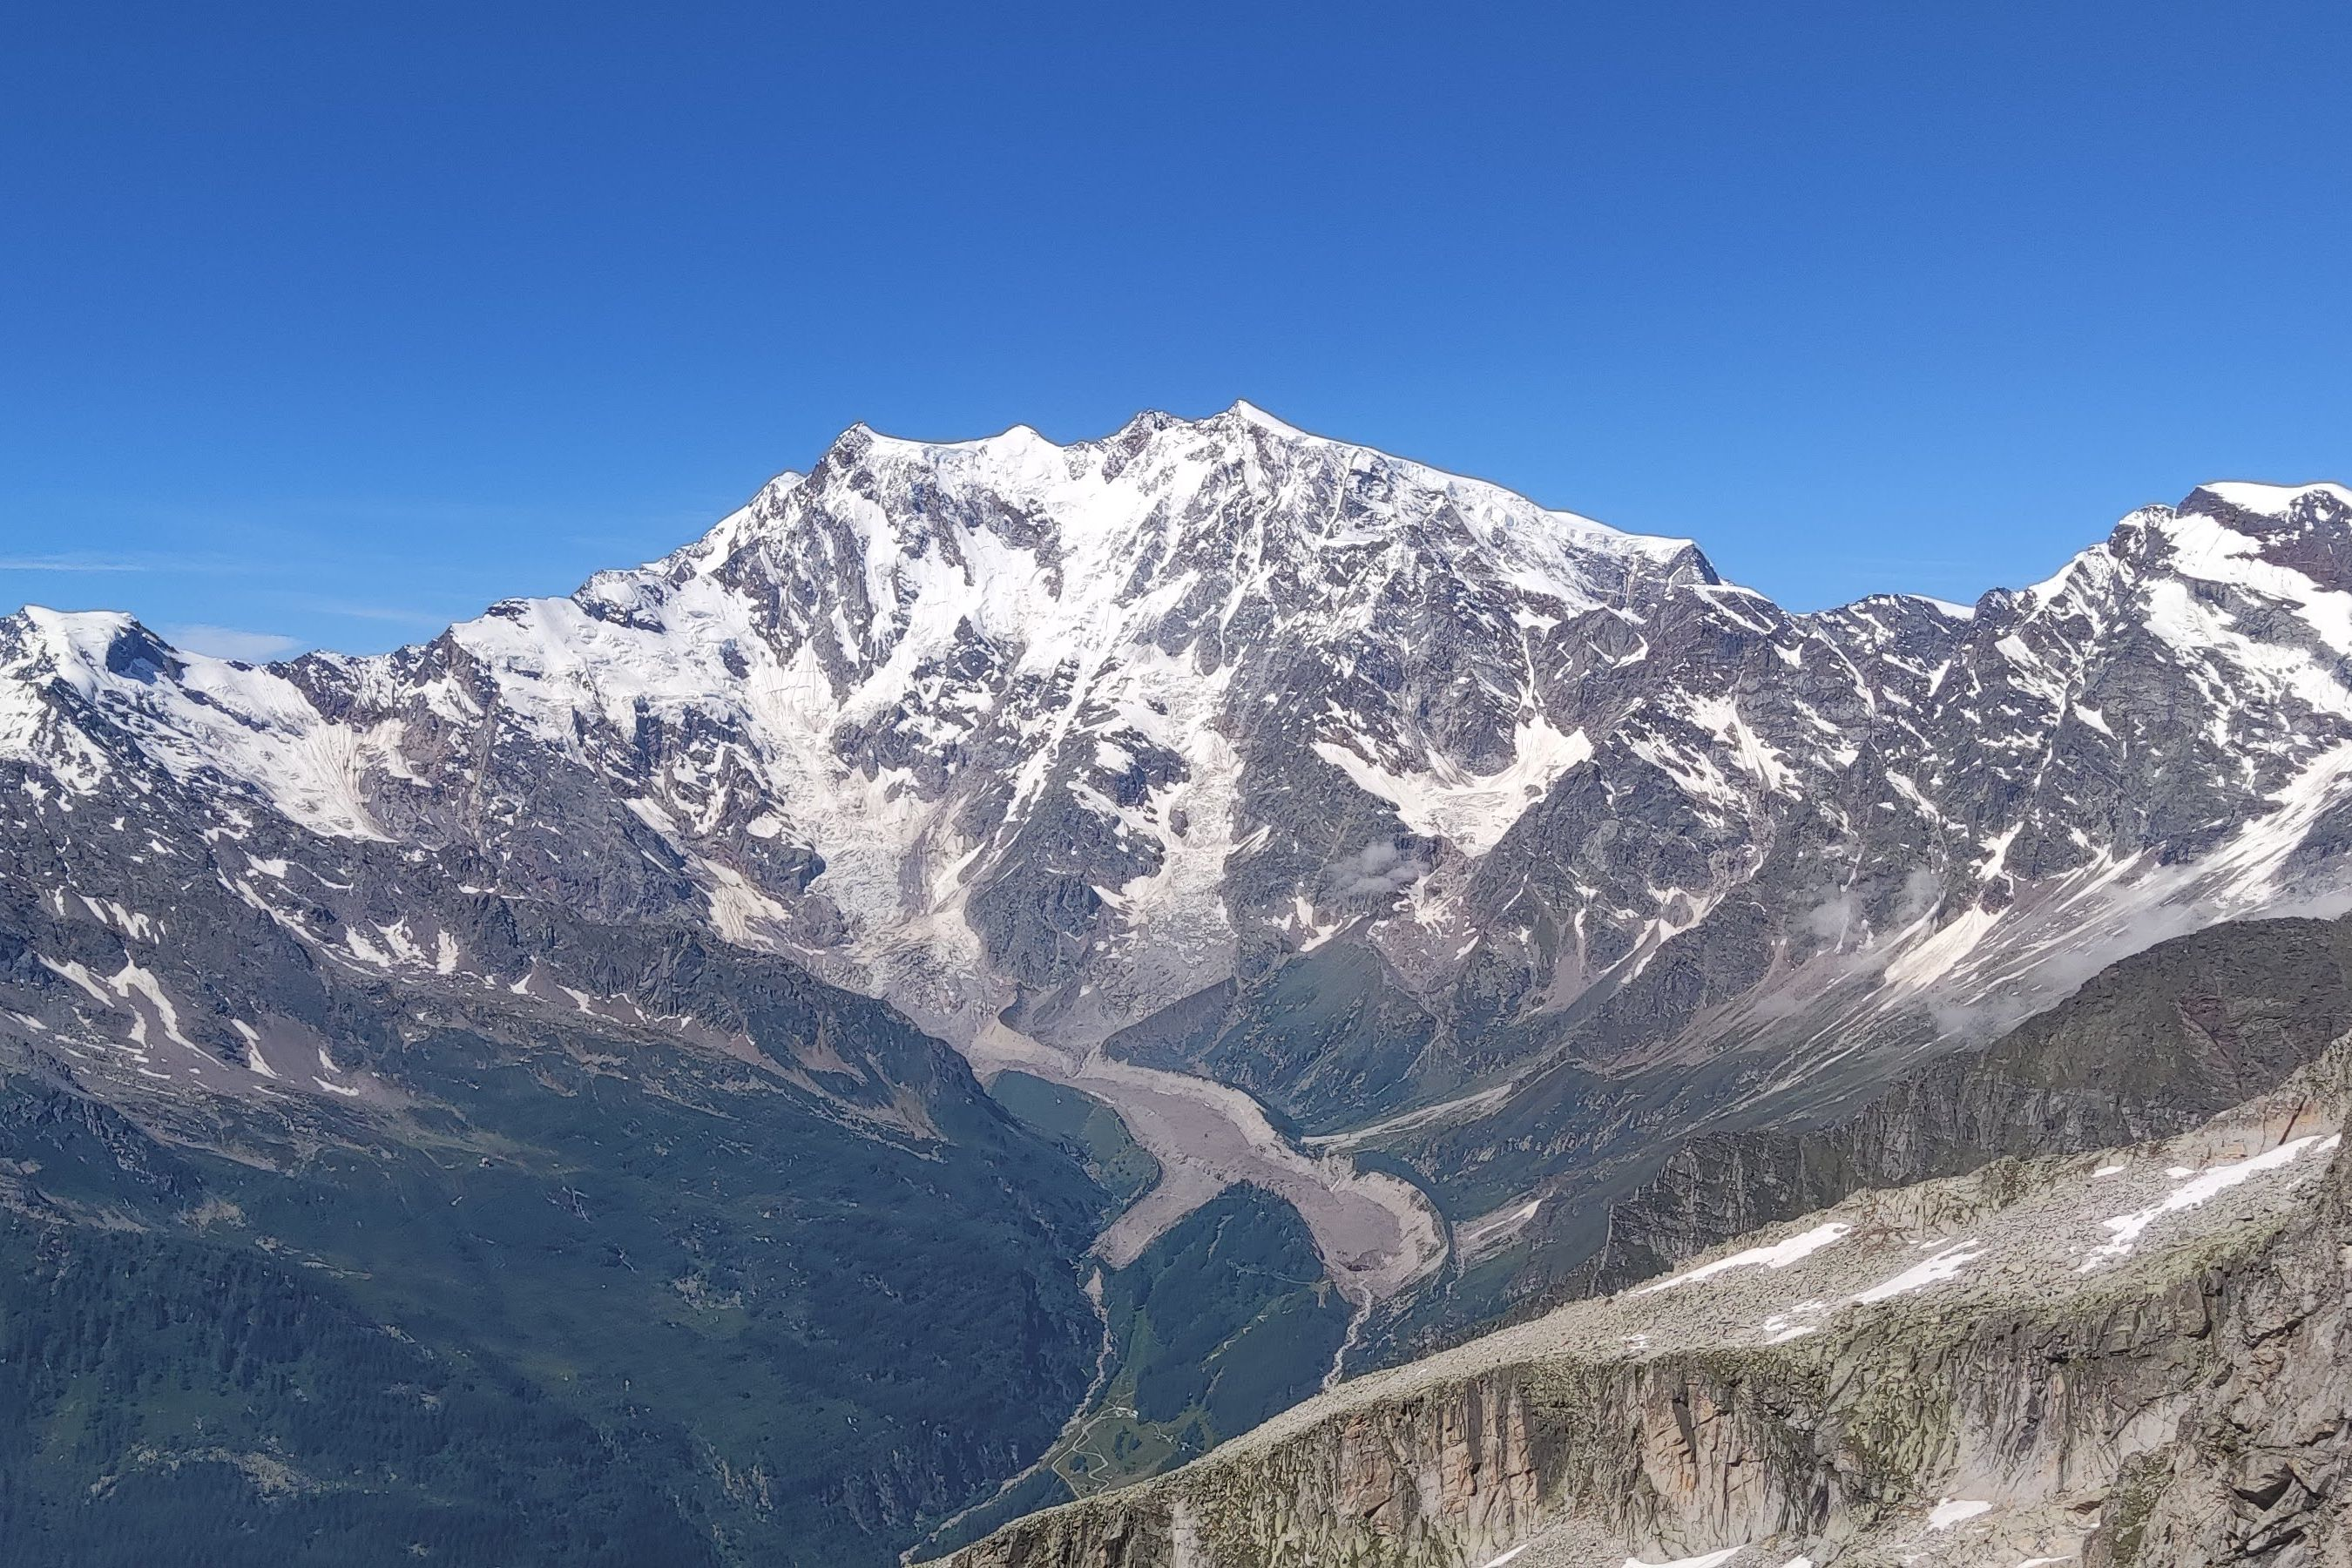
\includegraphics[height=5cm]{belvedere_pic.jpg}
    }
    \caption{(a) Location of Belvedere Glacier, base map (source: Swisstopo
        www.geo.admin.ch); (b) Picture of the Belvedere Glacier taken from the nearby Monte Moro.}
    \label{fig:1:studyarea}
\end{figure}

In the past, several hazardous events originated from the Belvedere Glacier, such as floods
and slope instability, threatened the nearby village of Macugnaga and the Zamboni Zappa
Hut, at 2070 m a.s.l. \citep{Kaab2004}.
At the beginning of the 21st century, the Belvedere Glacier was characterized by a
particular surge-type dynamics  \citep{Haeberli2002}.
During the late 1990s, the~surface speeds of the whole glacier were ranging between
\SIlist{30;45}{\meter\per\year}~\citep{Roethlisberger1985, Kaab2005}.
During 2000--2001, an accelerated flow in the Monte-Rosa Glacier produced a wave of
compression-decompression stresses and strains in the Belvedere Glacier.
Surface velocities soared: values up to \SI{200}{\meter\per\year} were observed
photogrammetrically during autumn 2001~\citep{Kaab2004}.
The ice thickness increased more than~\SI{20}{\meter} and the wave travelled downwards,
creating a depression area in the accumulation zone that was filled by a super-glacial
lake, the Lago Effimero~\citep{Haeberli2002, Mortara2009}.

During spring 2002, the large depression at the foot of the Monte Rosa east face, caused by the surge-type movement, was temporarily filled by a lake with a volume of \SI{3e6}{\cubic\meter}, the so-called \textit{Lago Effimero} (\textit{short-lived lake}).
Recognizing the potential danger of an outburst flood, the Italian Civil Defense Department rapidly 
implemented emergency measures, including evacuating parts of Macugnaga village, installing automatic 
alarm systems and pumps, and initiating detailed scientific investigations. 
Reduced meltwater input in July 2002, combined with natural subglacial drainage, stabilized and subsequently 
lowered the lake level.
However, the lake reformed in the spring of 2003, bursting out in mid-June without causing significant damage \citep{Kaab2004}.

% \textcolor{red}{Expand this part and add more pics with old and recent events}

% The northern lobe of the Belvedere Glacier is concurrently experiencing a fast retreat:
% in the past few years, an average retreat of \SI{\sim20}{\meter\per\year} was documented
% \citep{Ioli2022} and it is actively changing every day due to ice falls and collapses.


\section{Objectives}

This thesis explores the potential of multi-scale and multi-temporal photogrammetry 
for monitoring alpine glaciers, focusing on the debris-covered Belvedere Glacier in the Italian Alps.

This investigation integrates a spectrum of photogrammetric techniques.  
Firstly, historical aerial imagery analysis provides a long-term perspective on decades-long geomorphological changes at the meter scale.  
Secondly, in-situ UAV acquisitions enable annual reconstructions of glacier morphology, allowing for precise change analysis at a high spatial resolution.  
Finally, permanent in-situ monitoring using a low-cost stereo camera system allows for capturing the short-term dynamics of this rapidly changing environment.

% \textcolor{red}{Add figure of multi-temporal/multi-scale}

This study uses archival aerial photogrammetry data collected by public agencies during mapping flights to investigate the glacier's long-term evolution.
This technique allowed the reconstruction of past glacier morphology from 1977 to 2009, with approximately decadal intervals between models.  
The historical knowledge gained through this method is invaluable in documenting a natural heritage rapidly disappearing due to climate change. 
Of particular interest, archival photogrammetry reveals a significant period of glacier expansion in the early 21st century, allowing precise quantification of the increase in ice volume and glacier thickness.

This work integrates low-cost UAVs and GNSS for close-range photogrammetric monitoring to understand the glacier's current evolution.
Annual in-situ surveys since 2015 provide a periodic and highly accurate record of the evolution. 
Through these UAV surveys, centimeter-scale resolution enables detailed mapping of the dynamic environment, including precise quantification of glacier volume loss and study of variations in glacier flow rate.

However, alpine glacier dynamics are inherently non-linear, with a pronounced acceleration of processes in summer compared to winter.  
This trend has intensified in recent years due to the increasing frequency of hot and dry summers associated with climate change. 
While annual high-precision in-situ measurements provide essential insights into long-term geomorphological evolution, they lack the temporal resolution to fully capture the short-term kinematics of the glacier, which are crucial for
understanding the relationship between glacier dynamics and external drivers such as air temperature.
To address this need, a permanent monitoring system based on low-cost stereo cameras has been designed and installed on Belvedere Glacier. 
This system allows daily observations of glacier motion at a local spatial scale,
providing the high-frequency data needed for in-depth kinematic analysis.

This thesis describes the technical design and implementation of a low-cost glacier monitoring system and the development of novel software tools for extracting relevant information from stereo camera images via photogrammetric processing. 
A new pipeline was designed and published to overcome the limitations of existing software in handling images with extremely wide baselines. 
This pipeline allows the analysis of time-series point clouds and the extraction of metrics such as velocity, volume variations, and displacement.

The harsh mountain environment was a significant challenge, which constrained the camera placement.
This resulted in extremely wide baselines and significant viewpoint differences.  
These conditions made it difficult to find corresponding points using traditional local feature-matching techniques and hindered 3D reconstruction using existing commercial and open-source photogrammetric software.
To overcome this obstacle, a novel pipeline was developed using state-of-the-art deep-learning algorithms for robust feature matching that successfully overcomes the limitations of wide baseline stereo image processing.

This thesis presents a successful pilot test of the low-cost glacier monitoring system.
The current uses only two cameras installed at the northwest terminal lobe of the Belvedere glacier, focused on the terminal ice cliff, the portion of the glacier experiencing the most severe retreat and fast evolution. 
However, the system needs to be scaled up to achieve a more comprehensive and robust monitoring framework capable of capturing the glacier's entire dynamics. 
Expanding the camera network will increase the coverage and significantly improve the quality of daily 3D reconstructions through greater data redundancy.
Motivated by this potential, the final part of this thesis focuses on developing a flexible multi-view library. 
This library enables image matching using state-of-the-art deep learning algorithms and traditional handcrafted features. 
Crucially, it integrates seamlessly with existing photogrammetric software for streamlined 3D reconstruction, thus supporting the monitoring system's future expansion.


\section{Thesis outline}

This thesis is introduced in \textbf{\chref{ch:1}}. 
This chapter presents the motivation, the research problem, and the objectives of the thesis.
It introduces the Belvedere Glacier as a primary case study. It presents an overview of remote and close-range sensing techniques for alpine environments, focusing on image-based techniques for glacier monitoring at different spatial and temporal scales.

\textbf{\chref{ch:2}} analyzes the historical evolution of Belvedere Glacier (1977-2009) using archival aerial photogrammetry with sub-meter spatial resolution and decadal survey intervals.

\textbf{\chref{ch:3}} describes the annual UAV and GNSS survey methodology for contemporary monitoring of Belvedere Glacier (2015-2023).  
SfM-MVS techniques generate annual 3D models, orthophotos, and DSMs with decimeter resolution.
Glaciological analysis reveals complex spatial and temporal patterns in surface velocities, volume variations, and thinning effects.

\textbf{\chref{ch:4}} presents a novel low-cost stereo camera system for daily monitoring of a section of Belvedere Glacier (May-November 2022).
Deep learning algorithms overcome the challenges of large baselines, enabling accurate 3D reconstruction, surface velocity estimation, and quantification of ice loss with daily frequency. 

\textbf{\chref{ch:4}} describes Deep-Image-Matching (DIM), a novel open-source toolkit for wide-baseline, multi-view image matching in complex scenarios. 
DIM's robustness, flexibility, and integration capabilities make it a powerful tool for expanding the use of deep learning in photogrammetry. 

\textbf{\chref{ch:conclusion}} synthesizes the key findings of the thesis, highlighting their significance within glaciological research and the broader context of climate change.  
It emphasizes the unique long-term insights gained for Belvedere Glacier and the transformative tools developed for broader glacier monitoring. 
The commitment to open science and data sharing encourages collaboration and future research.

% References
\makechapterbibliography{}